\documentclass[10pt]{beamer}

\usetheme{Madrid}
\usecolortheme{beaver}

% =========================================
% BASIC PACKAGES
% =========================================
\usepackage{booktabs}       % Professional tables
\usepackage{array}          % Column types
\usepackage{multicol}       % Multi-column frames
\usepackage{amsmath}        % Mathematics
\usepackage{amssymb}        % Mathematical symbols
\usepackage{mdframed}       % Highlight boxes
\usepackage{ragged2e}

\usepackage[
    style=apa,
    backend=biber
]{biblatex}
\addbibresource{references.bib}

\hypersetup{
    pdftitle={Adaptive Gamification with Real-Time Harm Mitigation}
}

% Wrapping, left/center aligned table columns
\newcolumntype{L}[1]{>{\RaggedRight\arraybackslash}p{#1}}
\newcolumntype{C}[1]{>{\Centering\arraybackslash}p{#1}}

% Key-idea box
\definecolor{keyblue}{RGB}{0,61,122}
\newmdenv[
    linewidth=1pt,
    roundcorner=4pt,
    backgroundcolor=keyblue!8,
    linecolor=keyblue,
    innerleftmargin=5mm,
    innerrightmargin=5mm,
    innertopmargin=2.5mm,
    innerbottommargin=2.5mm
]{keybox}

% Compact itemize
\setbeamertemplate{itemize items}[circle]
\setlength{\parskip}{2pt}

\begin{document}

\title[Adaptive Harm-Aware Gamification]{Adaptive Gamification with Real-Time Harm Mitigation for Personalised Learning}
\subtitle{A Quasi-Experimental Research Proposal}
\author[Imran \quad Lee \quad Yaw]{
    \small IMRAN HARIS BIN MOHD AZLI (33\%) -- 252UC254P6\\[1pt]
    \small LEE CHONG CHUN (34\%) -- 252UC254YW\\[1pt]
    \small YAW YI WEOI (33\%) -- 251UC250TR
}
\institute[CPT6123]{
    \small Bachelor of Computer Science\\
    \small CPT6123 Research Method in Computer Science\\
    \small Lecturer: Jamal Arshad \quad|\quad Semester T2620
}
\date{30th September 2026}

\begin{frame}
\titlepage
\end{frame}

\begin{frame}{Outline}
\tableofcontents
\end{frame}


% =========================================
% 1. INTRODUCTION
% =========================================
\section{Introduction}

\begin{frame}{Gamification: documented gains, documented harms}
\begin{columns}[T]
    \column{0.48\textwidth}
    \begin{block}{Why it is used}
        \begin{itemize}
            \item Points, badges, leaderboards and challenges are now standard in learning platforms
            \item Meta-analysis of 22 studies: overall effect $g = 0.740$
            \item Knowledge $g = 0.841$, motivation $g = 0.743$ \cite{lu2024ai}
        \end{itemize}
    \end{block}
    \column{0.48\textwidth}
    \begin{alertblock}{What goes wrong}
        \begin{itemize}
            \item Performance pressure and leaderboard anxiety \cite{nugroho2025negative,edwards2022anxiety}
            \item Superficial point-chasing, declining intrinsic motivation
            \item Compulsive, notification-driven engagement \cite{gul2026brainrot}
            \item Same element, different meaning per learner \cite{gao2024sdt}
        \end{itemize}
    \end{alertblock}
\end{columns}
\vspace{0.3cm}
\begin{keybox}
\textbf{The difficulty:} one fixed configuration is applied to every learner, with no way to
detect harm -- or withdraw the element responsible -- while the learner is still engaged.
\end{keybox}
\end{frame}

\begin{frame}{What this proposal adds}
\begin{itemize}
    \item An \textbf{adaptive, harm-aware gamification controller}:
    \begin{itemize}
        \item estimate learner state (engagement, anxiety) from platform interaction traces
        \item compute a quantitative harm score $H_t$ against an individual threshold $\tau$
        \item keep, downgrade or substitute elements only while $H_t \le \tau$
    \end{itemize}
    \item A \textbf{semester-long quasi-experiment}: adaptive vs.\ static gamification vs.\
    non-gamified instruction, measuring benefit \emph{and} harm on the same weekly schedule
    \item Expected results: a validated state model, an operational harm metric, and tested
    element-configuration rules
\end{itemize}
\vspace{0.2cm}
\begin{keybox}
\textbf{The question in one line:} which configuration is safe for which learner, at which moment?
\end{keybox}
\end{frame}


% =========================================
% 2. LITERATURE REVIEW
% =========================================
\section{Literature Review}

\begin{frame}{Three themes, three research questions}
Builds on the group's critical research review of peer-reviewed studies from 2022--2025,
reorganised thematically rather than article by article:
\vspace{0.2cm}
\begin{columns}[T]
    \column{0.32\textwidth}
    \begin{block}{Theme 1 $\rightarrow$ RQ1}
        Adaptive and personalised gamification: how learner state is modelled and used.
    \end{block}
    \column{0.32\textwidth}
    \begin{block}{Theme 2 $\rightarrow$ RQ2}
        Documented negative effects and harm-mitigating design: what harms, from which elements.
    \end{block}
    \column{0.32\textwidth}
    \begin{block}{Theme 3 $\rightarrow$ RQ3}
        Evaluation designs and evidence: what is actually proven, and for how long.
    \end{block}
\end{columns}
\vspace{0.3cm}
\begin{keybox}
Each theme ends in a gap; the three gaps are the three research questions of this proposal.
\end{keybox}
\end{frame}

\begin{frame}{Theme 1: adaptive and personalised gamification (RQ1)}
\begin{itemize}
    \item Adaptive frameworks (e.g.\ Hexad typology) tailor mechanics to individual preferences
    \cite{zourmpakis2023adaptive,vistorte2024integrating}
    \item Learner-state models are updated from logs, questionnaires and multimodal signals;
    affective computing and deep learning predict states and cognitive needs
    \cite{vistorte2024integrating,naseer2025game}
    \item Runtime adaptation of game elements is technically feasible
    \cite{zourmpakis2023adaptive,shabadurai2025reinforcement}
    \item Yet the very elements used to engage -- badges, currency, forced cooperation -- can
    induce anxiety \cite{zourmpakis2023adaptive}
\end{itemize}
\vspace{0.1cm}
\begin{keybox}
\textbf{Gap for RQ1:} adaptation optimises engagement only. There is no real-time state model
tied to a validated feedback loop that can downgrade a harmful element. \cite{farhan2023machine}
\end{keybox}
\end{frame}

\begin{frame}{Theme 2: documented harms (RQ2)}
\begin{itemize}
    \item PRISMA review: 206 records screened, 20 studies retained, four harm categories --
    performance pressure, superficial learning, motivational decline, psychological distress
    \cite{nugroho2025negative}
    \item Harm is \textbf{element-specific}: leaderboards demotivate low-ranked learners,
    excessive challenge causes frustration, undirected feedback causes anxiety
    \item Language-learning review: anxiety examined in only 10 of 40 studies; competitive
    elements failed to reduce anxiety in half of the studies that used them \cite{edwards2022anxiety}
    \item Self-determination theory applied superficially -- the same element has a different
    \textbf{functional significance} for different learners \cite{gao2024sdt}
    \item Reward and notification loops drive compulsive engagement among 113 students
    \cite{gul2026brainrot}
\end{itemize}
\vspace{0.1cm}
\begin{keybox}
\textbf{Gap for RQ2:} harms are known as qualitative categories, not as a number a running
system can evaluate and enforce.
\end{keybox}
\end{frame}

\begin{frame}{Theme 3: evaluation evidence (RQ3)}
\begin{itemize}
    \item Quasi-experiments: gamified instruction beat traditional teaching over 4 weeks
    (136 students) \cite{zhang2026gamification}; gamified vs.\ non-gamified web development
    (60 students): performance up, engagement and motivation not significantly different
    \cite{ojonuba2025web}
    \item Four-month course (392 students): redesigned leaderboards and points reduced fear of
    failure and improved grades \cite{durmaz2022gamification}
    \item Cluster-randomised trial (217 computer science students): active learning outperformed
    lecture control \cite{lopezfernandez2024lego}
    \item Meta-analysis: $g = 0.740$ overall, and effects \textbf{shrink as the study period
    lengthens} \cite{lu2024ai,ming2025gamification}
\end{itemize}
\vspace{0.1cm}
\begin{keybox}
\textbf{Gap for RQ3:} short, single-condition, benefit-only designs -- adaptation is never the
treatment, and harm is never measured alongside benefit.
\end{keybox}
\end{frame}

\begin{frame}{Gap identification}
\begin{columns}[T]
    \column{0.32\textwidth}
    \begin{alertblock}{RQ1 gap}
        No real-time learner-state model, and no validated loop from estimated state to element
        selection.
    \end{alertblock}
    \column{0.32\textwidth}
    \begin{alertblock}{RQ2 gap}
        No operational harm metric that a system can compute online and enforce as a constraint.
    \end{alertblock}
    \column{0.32\textwidth}
    \begin{alertblock}{RQ3 gap}
        No long-duration, multi-condition study measuring benefit and harm on the same schedule.
    \end{alertblock}
\end{columns}
\vspace{0.3cm}
\begin{keybox}
The three gaps must be addressed \textbf{together}: a harm metric is only actionable if state
can be estimated in real time, and a state model is only meaningful if its output constrains
element selection.
\end{keybox}
\end{frame}


% =========================================
% 3. PROBLEM STATEMENT
% =========================================
\section{Problem Statement}

\begin{frame}{Context}
\begin{itemize}
    \item Gamification is a routine feature of platforms such as Kahoot! and Quizizz, which
    creates an implicit expectation that it is universally beneficial \cite{nugroho2025negative}
    \item Effectiveness is usually shown by short quasi-experiments: 3--4 teaching weeks, one
    fixed configuration, outcomes that omit anxiety \cite{zhang2026gamification,ojonuba2025web}
    \item Even the long evaluations stay single-condition -- four months varying only leaderboard
    and point designs \cite{durmaz2022gamification}
    \item Meta-analytic benefit ($g = 0.740$) must be read against equally systematic
    counter-evidence on pressure, anxiety and compulsive use
    \item One-size-fits-all rule systems cannot respond to frustration or disengagement as it
    occurs \cite{farhan2023machine,shabadurai2025reinforcement,naseer2025game}
\end{itemize}
\end{frame}

\begin{frame}{Gap}
\begin{enumerate}
    \item \textbf{Harms are categories, not quantities.} No study produces a numeric harm metric
    a running system can evaluate at decision time.
    \item \textbf{Mitigations are single-shot.} Relative leaderboards, cooperative structures,
    reduced gamification dose, digital detox -- all evaluated statically, none deployed as a
    closed-loop response to measured state \cite{nugroho2025negative,edwards2022anxiety,gao2024sdt,gul2026brainrot}.
    \item \textbf{Measurement is unbalanced.} Engagement is logged continuously; anxiety, need
    frustration and reward-chasing are measured rarely or not at all \cite{edwards2022anxiety}.
    \item \textbf{State models stay static.} Rigid typologies and basic metrics replace
    real-time affective estimation \cite{shabadurai2025reinforcement,zourmpakis2023adaptive,naseer2025game}.
\end{enumerate}
\vspace{0.1cm}
\begin{keybox}
A platform therefore cannot answer: which configuration minimises documented harm while
preserving engagement?
\end{keybox}
\end{frame}

\begin{frame}{Solution}
\begin{columns}[T]
    \column{0.55\textwidth}
    \begin{itemize}
        \item The controller \textbf{estimates} each learner's state from logs and brief
        self-report
        \item It \textbf{computes} a harm score $H_t$ over five constructs
        \item It \textbf{constrains} selection: apply a configuration only while
        $H_t \le \tau$, with $\tau$ calibrated to that learner's own baseline
        \item On violation, competitive and controlling elements are downgraded, and intensity
        is tapered as autonomous motivation grows \cite{gao2024sdt}
        \item It is \textbf{evaluated} over 14 weeks against static-gamified and non-gamified
        baselines with balanced benefit-and-harm metrics
    \end{itemize}
    \column{0.42\textwidth}
    \begin{keybox}\small
    \textbf{Rule:} apply a configuration only while $H_t \le \tau$\\[2pt]
    \textbf{Loop:} state $\rightarrow$ harm $\rightarrow$ constrained selection
    \end{keybox}
    \vspace{0.2cm}
    \begin{block}{Closes all three gaps}
    Supplies the harm constraint for RQ1, the metric for RQ2, and the treatment for RQ3.
    \end{block}
\end{columns}
\end{frame}


% =========================================
% 4. RESEARCH QUESTIONS
% =========================================
\section{Research Questions}

\begin{frame}{Research Questions}
\begin{enumerate}\itemsep6pt
    \item \textbf{RQ1:} How can learner state (engagement and anxiety) be modelled in real time
    to drive adaptive selection of gamification elements in an online learning platform?
    \item \textbf{RQ2:} Which gamification design configurations minimise documented negative
    effects -- anxiety, motivational undermining and superficial learning -- while preserving the
    engagement and achievement gains reported in the literature?
    \item \textbf{RQ3:} Does an adaptive, harm-aware gamification system improve learning
    outcomes and motivational quality compared with static gamification and non-gamified
    baselines over a full semester?
\end{enumerate}
\end{frame}


% =========================================
% 5. RESEARCH OBJECTIVES
% =========================================
\section{Research Objectives}

\begin{frame}{Research Objectives and Success Criteria}
\begin{columns}[T]
    \column{0.32\textwidth}
    \begin{block}{RO1 (RQ1)}
        A real-time learner-state model from interaction traces -- no EEG, no facial capture.
        \vspace{2pt}
        \begin{itemize}\itemsep0pt
            \item Disengagement AUC $\ge 0.75$
            \item Anxiety $r \ge 0.40$ with STAI-6
            \item Engagement $\ge$ static arm
        \end{itemize}
    \end{block}
    \column{0.32\textwidth}
    \begin{block}{RO2 (RQ2)}
        A quantitative harm metric $H_t$ plus pre-registered downgrade rules.
        \vspace{2pt}
        \begin{itemize}\itemsep0pt
            \item Cronbach's $\alpha \ge 0.70$
            \item Positive correlation with self-report
            \item Dry run never breaches $H_t \le \tau$
        \end{itemize}
    \end{block}
    \column{0.32\textwidth}
    \begin{block}{RO3 (RQ3)}
        A 14-week, three-arm evaluation with $\approx$150 undergraduates.
        \vspace{2pt}
        \begin{itemize}\itemsep0pt
            \item Harm $\ge 20\%$ lower than static
            \item Marks/sessions within 10\% margin
            \item Effects as Hedges' $g$ + 95\% CI
        \end{itemize}
    \end{block}
\end{columns}
\end{frame}


% =========================================
% 6. RESEARCH METHODOLOGY
% =========================================
\section{Research Methodology}

\begin{frame}{Design: three arms, one semester}
\begin{columns}[T]
    \column{0.52\textwidth}
    \begin{itemize}
        \item Quasi-experimental, \textbf{nonequivalent control-group} design, 14 weeks
        \item \textbf{A} adaptive harm-aware gamification\\
        \textbf{S} static gamification (one fixed configuration)\\
        \textbf{C} non-gamified instruction (same content, instructor, assessments)
        \item No random assignment: intact timetable classes are analysed as-is
        \item \textbf{Week 0} baseline: logging on, no elements yet $\rightarrow$ within-subject
        control for state and threshold
        \item Sample $\approx$150 learners ($\approx$50 per arm): 80\% power for $d \approx 0.56$
        \item Pre-registered analysis plan and downgrade rules
    \end{itemize}
    \column{0.45\textwidth}
    \begin{keybox}\footnotesize
    \textbf{Pipeline}\\
    \texttt{events $\rightarrow$ state}\\
    \texttt{$\rightarrow$ harm $\rightarrow$ selection}\\
    \texttt{$\rightarrow$ delivery $\rightarrow$ logging}
    \vspace{2pt}

    xAPI statements in an append-only event store; every decision is logged with its state
    estimate, harm score and applied configuration.
    \end{keybox}
    \vspace{0.2cm}
    \begin{block}{Attrition}\small
    Missing-at-random mixed-effects analysis plus a complete-case sensitivity check.
    \end{block}
\end{columns}
\end{frame}

\begin{frame}{Technical approach: the controller}
\begin{columns}[T]
    \column{0.55\textwidth}
    \begin{block}{Controller (per decision window)}
        \footnotesize
        \textbf{Input:} interaction stream $\mathbf{x}_t$, threshold $\tau$\\
        \textbf{Output:} element configuration $e_t$
        \vspace{2pt}
        \begin{enumerate}\itemsep1pt
            \item Estimate state $\hat{s}_t = f_\theta(\mathbf{x}_t)$ \hfill {\tiny engagement + anxiety}
            \item Compute harm $h(\hat{s}_t, e_{t-1})$
            \item \textbf{if} $h > \tau$ \textbf{then} downgrade competitive elements
            \item \textbf{else} $e_t \leftarrow \pi_\theta(\hat{s}_t)$
            \item Observe outcome; update $\theta$
        \end{enumerate}
    \end{block}
    \normalsize
    \vspace{0.1cm}
    Shipped as a Python service; each element emits its own exposure,
    response and abandonment events.
    \column{0.42\textwidth}
    \begin{block}{Replicable dry run}\small
        \begin{itemize}\itemsep1pt
            \item 20 simulated learners, 30 days, fixed seed 42
            \item Assert: applied configurations always satisfy $H_t \le \tau$
            \item Assert: the scheduled spike downgrades within one step
            \item Assert: a flat trace triggers no downgrade
        \end{itemize}
    \end{block}
\end{columns}
\end{frame}

\begin{frame}{Harm score and its validation}
\begin{columns}[T]
    \column{0.52\textwidth}
    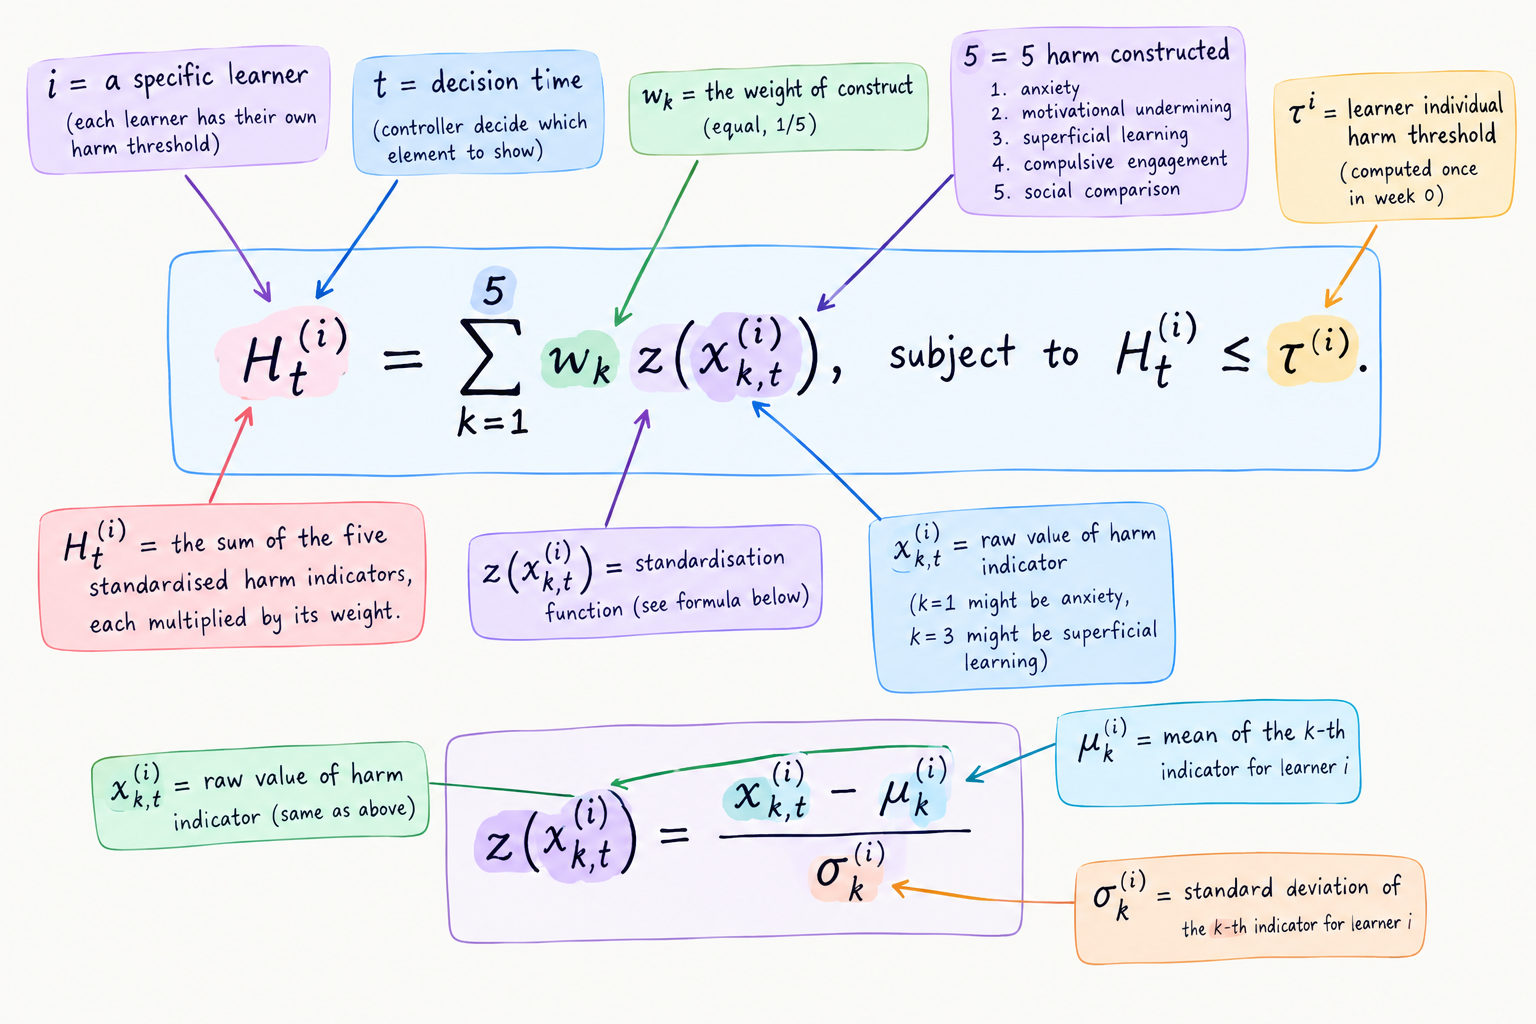
\includegraphics[width=\linewidth,keepaspectratio]{figure/formula.png}
    \par\vspace{3pt}
    \begin{center}\footnotesize The score each learner carries at decision time $t$:
    five standardised indicators, weighted and capped by their own threshold
    $\tau^{(i)}$.\end{center}
    \column{0.45\textwidth}
    \small
    \textbf{Five constructs} (higher = more harm):
    \begin{itemize}\itemsep0pt
        \item anxiety / psychological distress
        \item motivational undermining
        \item superficial learning
        \item compulsive engagement
        \item social comparison
    \end{itemize}
    \vspace{-6pt}
    \textbf{Calibration and checks:}
    \begin{itemize}\itemsep0pt
        \item Reverse-coded and standardised against each learner's own Week-0
        baseline ($H_t > 0$ = worse than own)
        \item Equal weights $w_k = 1/5$, pre-registered
        \item $\tau = \mu_{H_0} + \sigma_{H_0}$, fixed for the semester
        \item Validated with Cronbach's $\alpha$, self-report correlation, and
        24-hour session abandonment
    \end{itemize}
\end{columns}
\end{frame}

\begin{frame}{How each harm construct is measured}
\footnotesize
\begin{tabular}{|L{2.5cm}|L{5.0cm}|L{2.4cm}|}
\hline
\centering\textbf{Construct} & \centering\textbf{Operational variables / instrument} & \centering\textbf{Cadence}
\tabularnewline
\hline
Anxiety / distress & STAI-6 short form; stress-flag count; abandonment after a competitive display & Self-report Weeks 0, 6, 12; logs continuous
\tabularnewline
\hline
Motivational undermining & Need-frustration score; intrinsic motivation (reverse-coded); reward- vs.\ content-triggered action ratio & Waves Weeks 0, 6, 12; ratio weekly
\tabularnewline
\hline
Superficial learning & Reward-chasing ratio (reward screen time / task time); attempts without content review; transfer accuracy & Weekly + single-item prompt
\tabularnewline
\hline
Compulsive engagement & Sessions per day; session length; night activity (23:00--05:00); streak continuation; notification latency & Daily, 7-day rolling window
\tabularnewline
\hline
Social comparison & Leaderboard exposures; rank position; abandonment within 60\,s of a view & Event-triggered single item
\tabularnewline
\hline
\end{tabular}
\vspace{0.2cm}

\small Multi-item self-report only three times (burden control); log variables are used because
self-reported usage is biased \cite{gul2026brainrot}. All items oriented so higher = greater harm.
\end{frame}

\begin{frame}{Downgrade rules when $H_t > \tau$}
\footnotesize
\begin{tabular}{|L{2.6cm}|L{4.6cm}|L{2.6cm}|}
\hline
\centering\textbf{Element at risk} & \centering\textbf{Substitution or downgrade} & \centering\textbf{Evidence base}
\tabularnewline
\hline
Public leaderboard & Relative leaderboard (two ranks above/below) or cooperative group ranking & \textcite{nugroho2025negative}; \textcite{edwards2022anxiety}
\tabularnewline
\hline
Tangible points and rewards & Cap on reward magnitude; informational framing; progressive dose reduction & \textcite{gao2024sdt}; \textcite{nugroho2025negative}
\tabularnewline
\hline
Challenges & Difficulty adapted to demonstrated competence; otherwise add task-related choice & \textcite{gao2024sdt}
\tabularnewline
\hline
Feedback & Lower density; require directional guidance & \textcite{nugroho2025negative}
\tabularnewline
\hline
Levels / public progression & Show progress against the learner's own previous level; suspend public comparison & \textcite{nugroho2025negative}
\tabularnewline
\hline
Narrative and quests & \textbf{Prioritised, not downgraded} -- associated with lower anxiety & \textcite{edwards2022anxiety}
\tabularnewline
\hline
\end{tabular}
\vspace{0.2cm}

\small Rules are fixed before data collection; gamification is treated as a scaffold whose dose
is reduced as autonomous motivation develops \cite{gao2024sdt}.
\end{frame}

\begin{frame}{Evaluation criteria and analysis}
\begin{columns}[T]
    \column{0.48\textwidth}
    \textbf{Model criteria}
    \begin{itemize}\itemsep0pt
        \item Disengagement: AUC $\ge 0.75$ (plus precision, recall, F1)
        \item Anxiety: $r \ge 0.40$ with STAI-6 at Weeks 6 and 12
        \item Baselines: session-length logistic regression, last-value persistence
    \end{itemize}
    \vspace{0.1cm}
    \textbf{Metric criteria}
    \begin{itemize}\itemsep0pt
        \item $\alpha \ge 0.70$, positive self-report correlation, predicts abandonment above
        no-skill rate
    \end{itemize}
    \vspace{0.1cm}
    \textbf{Baselines and ablation}
    \begin{itemize}\itemsep0pt
        \item S = static configuration; C = no game elements
        \item Replayed ablations: constraint removed, and rule-based estimator -- never shown
        to a participant
    \end{itemize}
    \column{0.48\textwidth}
    \textbf{Outcome criteria (primary hypothesis)}
    \begin{itemize}\itemsep0pt
        \item A records weekly mean harm $\ge 20\%$ \textbf{lower} than S
        \item Marks and weekly sessions within a \textbf{10\%} non-inferiority margin of S
        \item Both gamified arms exceed C on knowledge gain and engagement
    \end{itemize}
    \vspace{0.1cm}
    \textbf{Analysis}
    \begin{itemize}\itemsep0pt
        \item Linear mixed-effects models, random intercepts for learner and week
        \item Effect sizes with 95\% CI; non-inferiority at $\alpha = 0.05$; multiple-comparison
        correction
        \item Decision latency $< 1$\,s; full model coverage of active learners
    \end{itemize}
\end{columns}
\end{frame}

\begin{frame}{Ethical considerations}
\begin{itemize}
    \item \textbf{Approval and consent:} submitted to the university ethics committee before
    recruitment; voluntary participation, written consent, withdrawal deletes that record
    \item \textbf{No academic disadvantage:} control arm receives identical content,
    assessment and instructor contact; gamification contributes \textbf{no course marks}
    \item \textbf{Data protection:} minimised, pseudonymised, encrypted, access-controlled;
    Malaysian PDPA 2010; raw logs retained three years then destroyed; results only in aggregate
    \item \textbf{Non-maleficence by design:} $\tau$ is a hard constraint inside the controller,
    so a harm-raising configuration cannot be selected; no streak-loss or negative-notification
    mechanics \cite{gul2026brainrot}
    \item \textbf{Bias control:} harm rates monitored across subgroups; leaderboard visibility
    opt-in (default = relative/cooperative) \cite{edwards2022anxiety}; all decisions logged and
    auditable, rules pre-registered
\end{itemize}
\end{frame}


% =========================================
% 7. EXPECTED OUTCOMES
% =========================================
\section{Expected Outcomes}

\begin{frame}{Expected outcomes and deliverables}
\begin{columns}[T]
    \column{0.55\textwidth}
    \begin{enumerate}\itemsep4pt
        \item \textbf{A validated real-time learner-state model} -- AUC $\ge 0.75$,
        $r \ge 0.40$ with STAI-6, no EEG or facial capture
        \item \textbf{An operational harm metric} -- $H_t$ computable at decision time, with
        individualised $\tau$, three validation checks and pre-registered weights
        \item \textbf{Tested element-configuration rules} -- evidence on whether harm falls by
        $\ge 20\%$ while marks stay within a 10\% margin
        \item \textbf{A semester-long three-arm comparison} -- benefit and harm measured on the
        same weekly schedule over 14 weeks
    \end{enumerate}
    \column{0.42\textwidth}
    \begin{block}{Deliverables}
        \begin{itemize}\itemsep0pt
            \item Instrumented LMS plugin and controller source code
            \item Pre-registered analysis plan
            \item De-identified dataset with data dictionary
            \item Reproducibility package
            \item $\ge 1$ manuscript submitted to a peer-reviewed venue
        \end{itemize}
    \end{block}
    \vspace{0.2cm}
    \begin{keybox}
    A shift from \emph{whether} gamification works to \emph{which configuration is safe for
    which learner at which moment}.
    \end{keybox}
\end{columns}
\end{frame}


% =========================================
% 8. PROJECT TIMELINE
% =========================================
\section{Project Timeline}

\begin{frame}{Project timeline}
\footnotesize
\begin{tabular}{|L{2.6cm}|L{3.4cm}|L{1.6cm}|L{2.4cm}|}
\hline
\centering\textbf{Phase} & \centering\textbf{Activities} & \centering\textbf{Duration} & \centering\textbf{Milestone}
\tabularnewline
\hline
1. Requirement \& design & Gap analysis, system specification, ethics submission & Days 1--14 & Design document, ethics approval
\tabularnewline
\hline
2. Modelling \& prototyping & Learner-state model, harm metric, controller prototype & Days 15--45 & Working prototype
\tabularnewline
\hline
3. Pilot \& refinement & Synthetic dry run, pilot run, metric calibration & Days 46--60 & Pilot report
\tabularnewline
\hline
4. Full evaluation & Three-arm deployment: 7-day baseline + 98 days of data collection & Days 61--165 & Complete dataset
\tabularnewline
\hline
5. Analysis \& write-up & Mixed-effects analysis, ablation, write-up & Days 166--195 & Results \& manuscript
\tabularnewline
\hline
\end{tabular}
\vspace{0.3cm}

\normalsize The 105-day evaluation window (Days 61--165) = 7-day baseline + the 14-week
intervention.
\end{frame}


% =========================================
% 9. CONCLUSION
% =========================================
\section{Conclusion}

\begin{frame}{Conclusion}
\begin{columns}[T]
    \column{0.52\textwidth}
    \begin{itemize}
        \item Benefits of gamification are well documented; so are its harms
        \item Yet no system measures harm as a quantity, reacts while the learner is engaged,
        or is evaluated against benefit \emph{and} harm together
        \item The proposal closes the loop: state model $+$ individualised $H_t \le \tau$
        $+$ pre-registered downgrade rules, tested over 14 weeks in three arms
        \item Expected: valid state model, valid harm metric, harm $\ge 20\%$ lower than static
        with gains held within 10\%
    \end{itemize}
    \column{0.45\textwidth}
    \begin{keybox}
    \textbf{Gamification does not need to be abandoned -- it needs to be governed.}
    \end{keybox}
    \vspace{0.1cm}
    Measurable, constrainable harms turn the ethical principle of non-maleficence into an
    engineering requirement.
    \vspace{0.1cm}
    \begin{alertblock}{The question is no longer whether game elements motivate, but whether a
    system can detect when it is doing harm -- and act on that knowledge before the learner
    disengages.}
    \end{alertblock}
\end{columns}
\end{frame}


% =========================================
% REFERENCES
% =========================================
\begin{frame}[allowframebreaks]{References}
\renewcommand*{\bibfont}{\footnotesize}
\setlength{\bibitemsep}{1.5pt}
\printbibliography
\end{frame}

\end{document}
